
\def\lecturetitle{Comunicação entre processos ({\em Interprocess
    Communication -- IPC})}
\part{\lecturetitle}

\frame{\title{\lecturetitle}\titlepage}

\frame{\frametitle{Trilha}\tableofcontents[part=1]}

\def\proc{\tiny{processo}}
\def\init{-5}
\def\xshifti{4pt} % interprocesses
\def\xshiftp{3pt} % between interprocesses

\def\thetitle{Introdução}
\section{\thetitle}

\begin{frame}{POSIX}{Padrões Unix}

POSIX ({\em Portable Operating System Interface})

\begin{itemize}
\item Conjunto de padrões em desenvolvimento pelo {\em Institute for
    Eletrical and Electronical Engineers} (IEEE), também sendo
  adotados pela ISO ({\em International Organization for
    Standardization}) e IEC ({\em International Electrotechnical
    Comission}).
\item Alguns padrões:
  \begin{itemize}
  \item IEEE Std 1003.1 -- 1990: linguagem C;
  \item IEEE Std 1003.2 -- 1992: {\em shell} e outros utilitários;
  \item IEEE Std 1003.1b -- 1996: sincronização de arquivos, E/S
    assíncrona, semáforos, gerenciamento de memória, relógios e
    temporizadores, escalonamento, dentre outros.
  \end{itemize}
\item Exemplos: chamadas de sistema {\tt fork}, {\tt open}, {\tt close}.

\end{itemize}
  
\end{frame}


\begin{frame}
\frametitle{Processos, {\em threads} e compartilhamento de
  dados\footnote{\tiny Fonte: ``Unix Network Programming, Interprocess
    Comunication''. W. R. Stevens, 1998.}}
\framesubtitle{Por quê se comunicar?}

\begin{tikzpicture}[proc/.style={draw,rectangle},
  mem/.style={draw,rectangle,red!70!black},
  fs/.style={draw,shape=rectangle,red!70!black},
  infoline/.style={draw,<->,dashed}]
  
  \node[proc] (proc1) at (\init,0) {\proc};
  \node[proc] (proc2) [right of=proc1,xshift=\xshifti] {\proc};
  \node[fs] (fs) at (\init+0.5,-4) {\tiny{sistema de arquivos}};
  \only<2->{
    \draw[<->] (proc1) -- (fs);
    \draw[<->] (fs) -- (proc2);
  }

  \node[proc] (proc3) [right =of proc2] {\proc};
  \node[proc] (proc4) [right =of proc3,xshift=-6*\xshifti] {\proc};
  \node[proc,red!70!black] (info) [below
  of=proc3,yshift=-7.9*\xshiftp,xshift=4.5*\xshiftp] {\tiny{informação
      compartilhada}};
  \only<3->{
    \draw[<->] (proc3) -- (info);
    \draw[<->] (info) -- (proc4);
  }

  \node[proc] (proc5) [right =of proc4,xshift=\xshifti] {\proc};
  \node[mem] (mem) [right =of proc5,xshift=-8*\xshiftp] {\tiny{$\frac{memoria}{compartilhada}$}};
  \node[proc] (proc6) [right =of mem,xshift=-8*\xshiftp] {\proc};
  
  \only<4->{
    \path[infoline] (proc5) -- ++(0,-0.5) -- ++(1.4,0) -- (mem);
    \draw[infoline] (mem) -- ++(0,-0.5) -- ++(1.4,0) -- (proc6);
  }

  \draw[dashed,blue!70!black] (\init-1, -2.5) node[anchor=south west,blue!70!black]{\small{kernel}} rectangle (5.35, -1);

  \only<5->{
    \node[anchor=west] at (\init+3,-5) {Compartilhamento de recursos (\alert{dados})!};
  }

\end{tikzpicture}

\end{frame}


\def\thetitle{Mecanismos de IPC}
\section{\thetitle}
\frame{\author{}\institute{}\date{}\title{\thetitle}\titlepage}

\begin{frame}{Principais mecanismos de IPC}

  \begin{itemize}
  \item {\em Pipes};
  \item Mensagens;
  \item Memória compartilhada;
  \item Semáforos;
  \item Sinais.
  \end{itemize}
  
\end{frame}

\begin{frame}{Pipes}
  \small Propiciam comunicação síncrona entre os processos tendo
  descritores de arquivos ({\em file descriptor -- fd}) como interface
  entre os
  processos e o kernel que gerencia a comunicação.\\
  \smallskip
  Exemplo:\\
\begin{center}
  figure
  \begin{center}
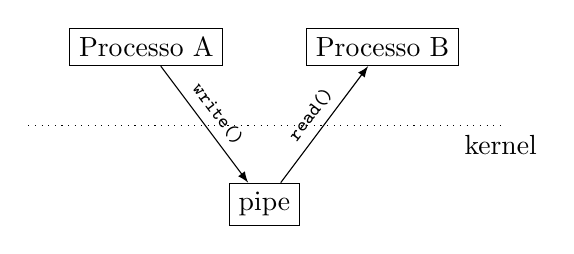
\begin{tikzpicture}
\def\shift{3cm}
\def\yshift{\shift/3}
\tikzset{base/.style={draw},pipe/.style={base},proc/.style={base},
every path/.style={>=latex,draw},syscal/.style={font=\scriptsize\tt}}
\node[pipe] at (\shift,-\yshift) (PIPE) {pipe};
\draw[dotted] (0,0) -- (2*\shift,0) node[below] {kernel};
\node[proc] at (\shift/2,\yshift) (PA) {Processo A};
\node[proc] at (1.5*\shift,\yshift) (PB) {Processo B};
\path[->] (PA) -- node[syscal,rotate=-53,above]{write()} (PIPE);
\path[->] (PIPE) -- node[syscal,rotate=53,above]{read()} (PB);
\end{tikzpicture}
\end{center}

\end{center}

API Posix $\rightarrow$ {\tt int pipe(int fd[2]);}

\end{frame}

\begin{frame}{Sinais}
  
  Um sinal é uma mensagem enviada diretamente ao processo.
  \vspace{1.5cm}

  \begin{columns}
     \begin{column}{.5\textwidth}

  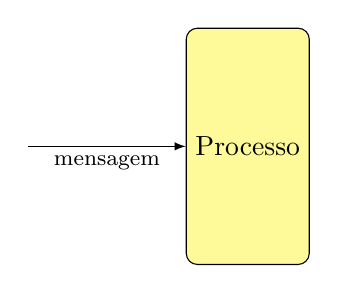
\begin{tikzpicture}
    \tikzset{proc/.style={rounded corners,minimum height=3cm,draw}}
    
    \node[proc,anchor=west,fill=yellow!40] at (2,1) (proc) {Processo};
    \draw[->,>=latex] (0,1) -- (2,1) node[anchor=north,midway] {\footnotesize mensagem};
  \end{tikzpicture}
\end{column}

\begin{column}{.5\textwidth}
  \small
  Exemplo:\\
  \# comando {\sc Unix} para para um processo rodando com PID
    4123\\
    \bigskip
  {\tt \$ kill -SIGHUP 4123}

  

\end{column}      

\end{columns}

\end{frame}

\begin{frame}{Memória compartilhada}
  
  \begin{center}
    \begin{center}
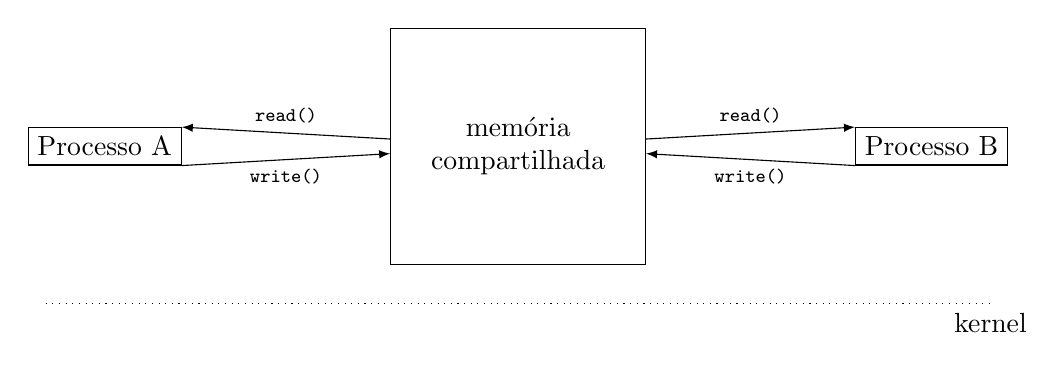
\begin{tikzpicture}
\def\shift{3cm}
\def\yshift{\shift/1.5}
\tikzset{base/.style={draw},
mem/.style={base,minimum width=\shift,minimum height=\shift,align=center},
proc/.style={base},
every path/.style={>=latex,draw},syscal/.style={font=\scriptsize\tt}}
\node[mem,text width=\shift] at (0,0) (MEM) {memória\\ compartilhada};
\node[proc] at (-1.75*\shift,0) (PA) {Processo A};
\node[proc] at (1.75*\shift,0) (PB) {Processo B};
\path[->] (PA.south east) -- node[syscal,below]{write()} (MEM);
\path[->] (MEM) -- node[syscal,above]{read()} (PA.north east);
\path[->] (MEM) -- node[syscal,above]{read()} (PB.north west);
\path[->] (PB.south west) -- node[syscal,below]{write()} (MEM);
\draw[dotted] (-2*\shift,-\yshift) -- (2*\shift,-\yshift) node[below] {kernel};
\end{tikzpicture}
\end{center}

  \end{center}

\end{frame}

\begin{frame}
  \frametitle{Mensagens}
  \framesubtitle{Comunicação assíncrona}
  \small
  Dois ou mais processos podem se comunicar utilizando um sistema
  comum de fila de mensagens.

  \begin{center}
  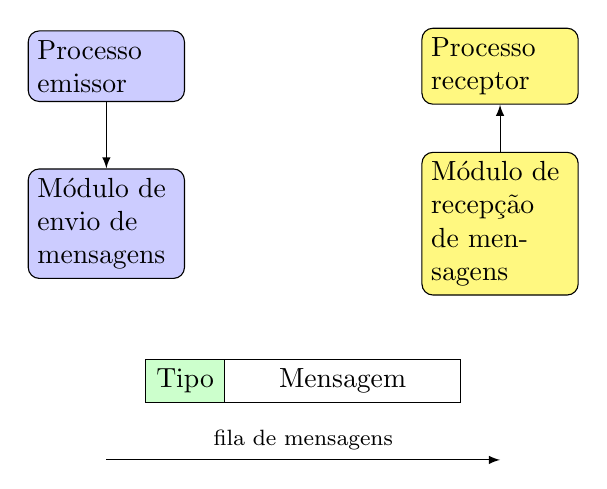
\begin{tikzpicture}
    \tikzset{mod/.style={rounded corners,text width=1.75cm,draw},
    send/.style={fill=blue!20},rec/.style={fill=yellow!50}}
    \node[mod,send] (sp) {Processo emissor};%sending process
    \node[mod,rec] (rp) [right of=sp,xshift=40mm] {Processo
      receptor};%receiving process
    \node[mod,send] (mps) [below of=sp,yshift=-10mm] {Módulo de envio de mensagens};
    \node[mod,rec] (mpr) [below of=rp,yshift=-10mm] {Módulo de recepção de
      mensagens};
    \node[draw,minimum width=1cm,fill=green!20] (type) [below of=mps,yshift=-10mm,xshift=10mm] {Tipo};
    \node[draw,minimum width=3cm] (mesg) [right of=type,xshift=10mm] {Mensagem};
    
    \draw[->,>=latex] (sp) -- (mps);
    \draw[<-,>=latex] (rp) -- (mpr);
    \draw[->,>=latex] (0,-5) -- (5,-5);
    \node at (2.5,-4.75) {\footnotesize fila de mensagens};
  \end{tikzpicture}
\end{center}

API Posix para:\\
 \alert{enviar} mensagens $\rightarrow$ {\tt int mq\_send();}\\
\alert{receber} mensagens $\rightarrow$ {\tt int mq\_receive();}

\end{frame}

